\documentclass{article}

\usepackage{graphicx}
\usepackage{tikz}
\usepackage{tikzsymbols}
\usetikzlibrary{calc,patterns,shapes.geometric}
\pagestyle{empty}
\usepackage[margin=0pt]{geometry}
\geometry{papersize={14in,12in}}

\def\centerarc[#1](#2)(#3:#4:#5){\draw[#1] ($(#2)+({#5*cos(#3)},{#5*sin(#3)})$) arc (#3:#4:#5);}

\begin{document}
	\begin{figure}
		\centering
		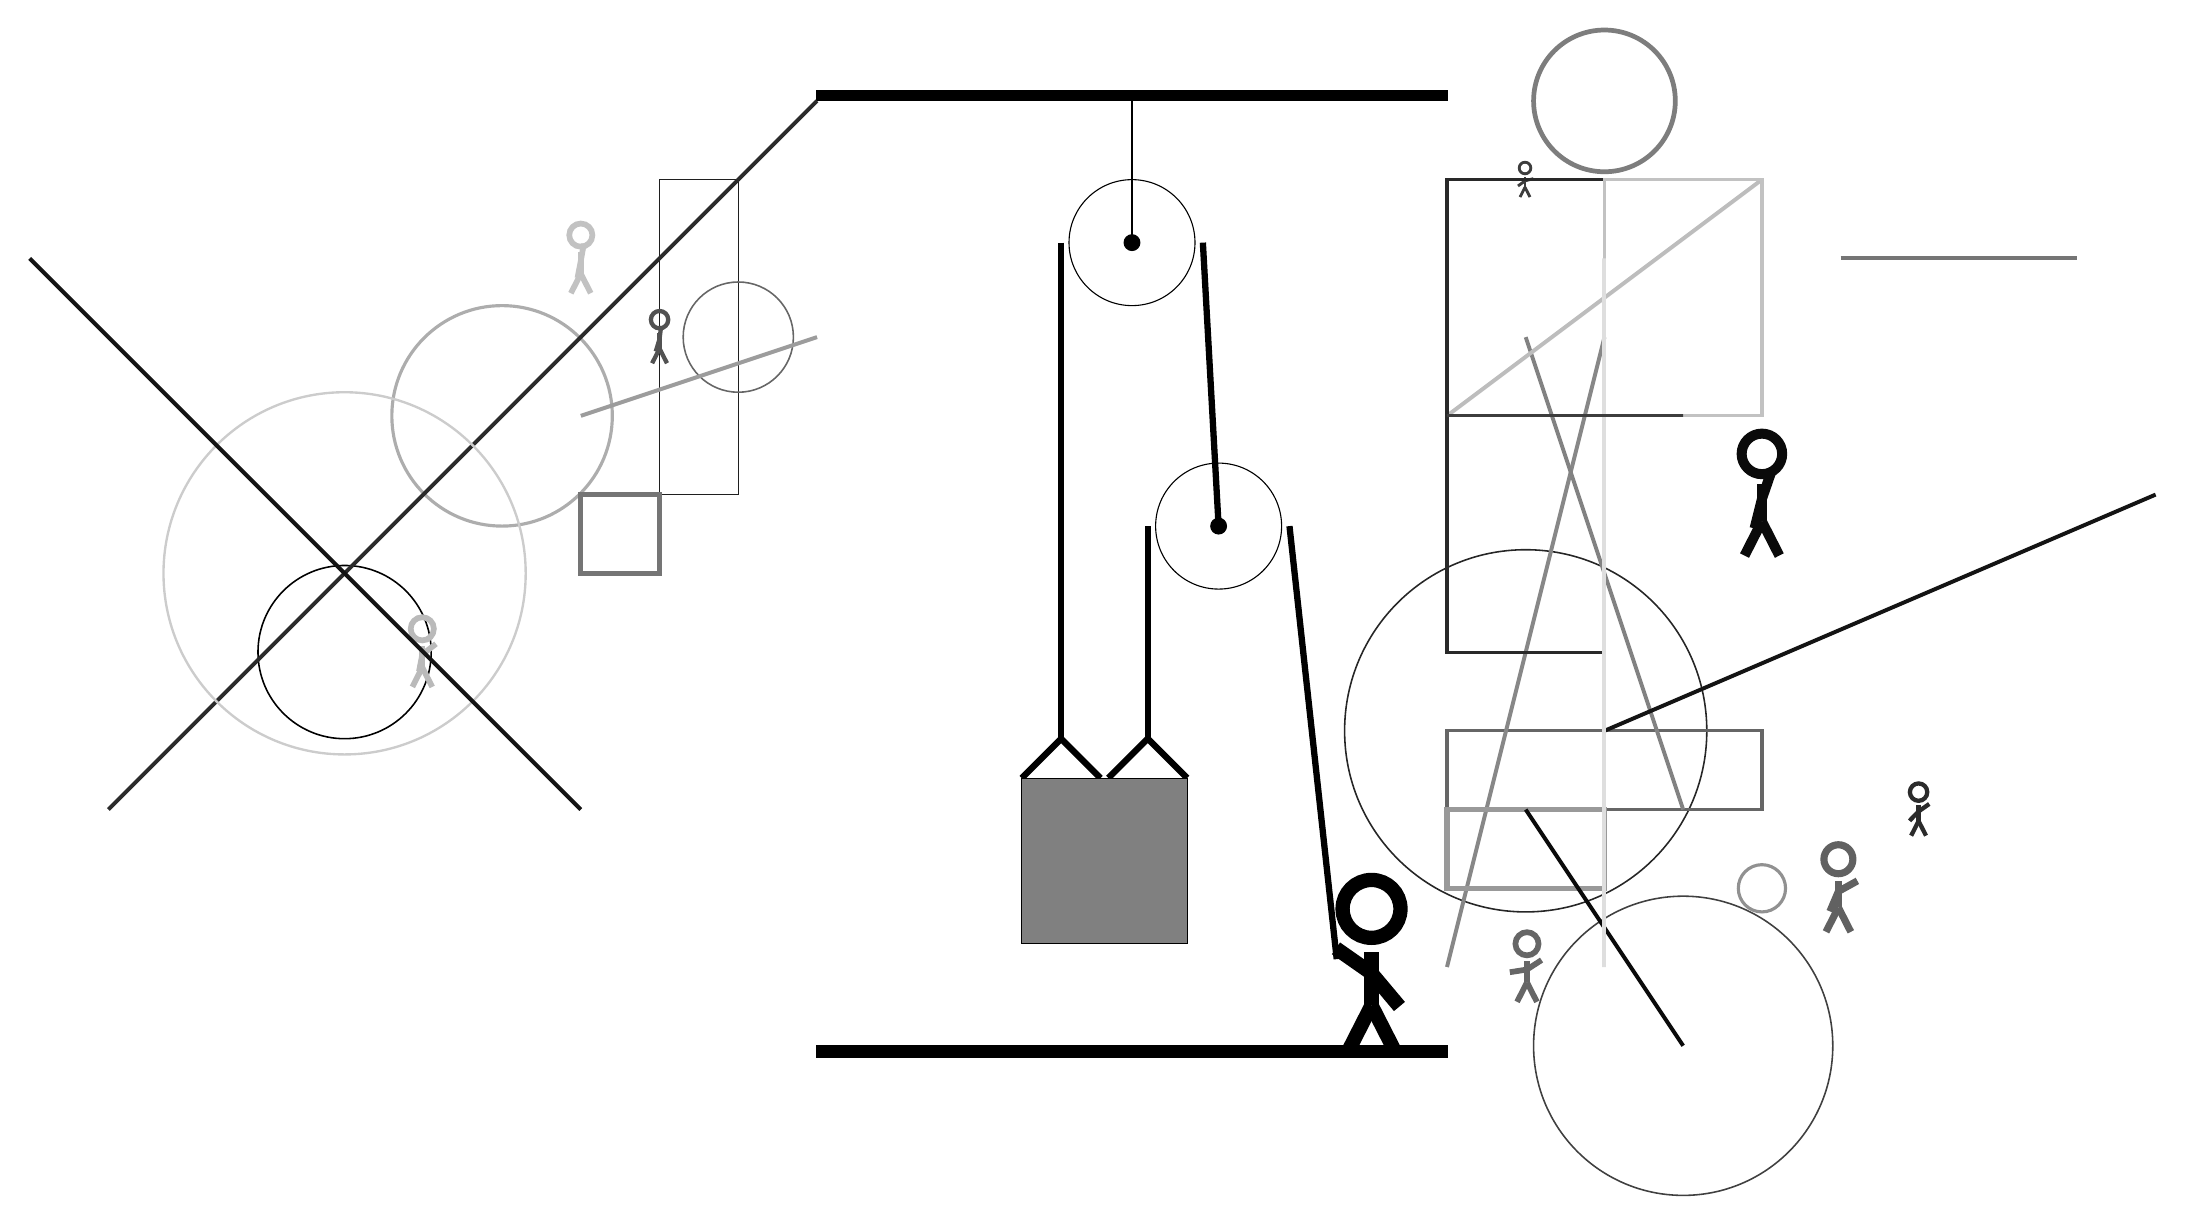
\begin{tikzpicture}
			%%%%% START %%%%%
			
			\draw[fill=black] (-2, 9) rectangle (6, 9.125);
			
			\draw (2, 7.2) circle (0.8);
			\draw[fill=black] (2, 7.2) circle (0.1);
			\draw[thick] (2, 7.2) -- (2, 9);
			
			\draw [line width=0.6mm, color=black!51](8, 9) circle (0.9);
			
			\draw [line width=0.2mm, color=black!85](7, 1) circle (2.3);
			\draw [line width=0.4mm, color=black!32](-6, 5) circle (1.4);
			\draw [line width=0.2mm, color=black!75](9, -3) circle (1.9);
			\draw[line width=0.4mm, color=black!60] (6, 0) rectangle (10, 1);
			
			\draw[line width=0.2mm, color=black!88] (-4, 8) rectangle (-3, 4);
			
			\draw[line width=0.5mm, color=black!47](8, 6) -- (6, -2);
			\draw[line width=0.6mm, color=black!54] (-4, 4) rectangle (-5, 3);
			\draw[line width=0.5mm, color=black!49](9, 0) -- (7, 6);
			\draw[line width=0.7mm, color=black!40] (8, -1) rectangle (6, 0);
			\draw[line width=0.5mm, color=black!96](9, -3) -- (7, 0);
			\node[line width=0.7mm, color=black!96] at (10, 4) {\Strichmaxerl[7][76][71]};
			\draw[line width=0.5mm, color=black!92](8, 1) -- (15, 4);
			
			\draw [line width=0.2mm, color=black!60](-3, 6) circle (0.7);
			\draw[line width=0.5mm, color=black!26](10, 8) -- (6, 5);
			\draw [line width=0.2mm, color=black!100](-8, 2) circle (1.1);
			\draw [line width=0.4mm, color=black!43](10, -1) circle (0.3);
			
			\node[line width=0.3mm, color=black!24] at (-5, 7) {\Strichmaxerl[4][79][80]};
			\node[line width=0.3mm, color=black!76] at (7, 8) {\Strichmaxerl[2][36][15]};
			\draw[line width=0.4mm, color=black!84] (6, 2) rectangle (8, 8);
			\draw[line width=0.5mm, color=black!54](11, 7) -- (14, 7);
			
			\draw[line width=0.5mm, color=black!39](-5, 5) -- (-2, 6);
			
			\node[line width=0.6mm, color=black!62] at (11, -1) {\Strichmaxerl[5][67][29]};
			\node[line width=0.7mm, color=black!27] at (-7, 2) {\Strichmaxerl[4][79][38]};
			\draw[line width=0.4mm, color=black!24] (8, 5) rectangle (10, 8);
			\draw[line width=0.5mm, color=black!13] (8, -2) rectangle (8, 7);
			
			\draw[line width=0.4mm, color=black!76] (6, 5) rectangle (9, 5);
			\draw[line width=0.5mm, color=black!83](-2, 9) -- (-11, 0);
			
			\node[line width=0.2mm, color=black!83] at (12, 0) {\Strichmaxerl[3][46][35]};
			
			\draw [line width=0.3mm, color=black!20](-8, 3) circle (2.3);
			\node[line width=0.7mm, color=black!68] at (-4, 6) {\Strichmaxerl[3][73][83]};
			\node[line width=0.7mm, color=black!60] at (7, -2) {\Strichmaxerl[4][9][33]};
			\draw[line width=0.5mm, color=black!92](-5, 0) -- (-12, 7);
			
			
			\draw (3.1, 3.6) circle (0.8);
			\draw[fill=black] (3.1, 3.6) circle (0.1);
			
			\draw[line width = 0.8mm]  (0.6, 0.4) -- (1.1, 0.9) -- (1.6, 0.4);
			\draw[line width = 0.8mm]  (1.7, 0.4) -- (2.2, 0.9) -- (2.7, 0.4);
			\draw[fill=black!50] (0.6, 0.4) rectangle (2.7, -1.7);
			
			\draw[line width = 0.8mm] (1.1, 7.2) -- (1.1, 0.9);
			\centerarc[line width = 0.8mm](2, 7.2)(0:180:0.9);
			\draw[line width = 0.8mm] (2.9, 7.2) -- (3.1, 3.6);
			\draw[line width = 0.8mm] (2.2, 3.6) -- (2.2, 0.9);
			\centerarc[line width = 0.8mm](3.1, 3.6)(0:180:0.9);
			\draw[line width = 0.8mm] (4.0, 3.6) -- (4.6, -1.9);
			
			\node at (5, -2) {\Strichmaxerl[10][-35][-50]};
			
			\draw[fill=black] (-2, -3) rectangle (6, -3.15);
			
			%%%%% END %%%%%
		\end{tikzpicture}
	\end{figure}	
\end{document}